\subsection{Implementierung der klassischen MC-Methode}
In diesem Kapitel sei $l=10$. Insbesondere ist also $m_l=2^{10}$.
Ich habe die klassische Monte-Carlo-Methode in  Matlab implementiert. In folgender Tabelle sind die erhaltenen Ergebnisse zu verschiedenen $\lambda$ und ansteigender Anzahl an Samples $n$ aufgelistet.
\begin{center}
\begin{tabular}{|l|c|c|c|c|c|r|}
\hline
\diagbox{$n$}{$\lambda$} & 0.3 &0.5&0.7&1  \\ 
 \hline 
50  &  0.2000 &   0.4000  &  0.5200 &   0.6800\\
100    & 0.2400 &   0.3900  &  0.5200  &  0.6500\\
200    & 0.2100  &  0.3000  &  0.4400  &  0.6650\\
500    &  0.1980 &   0.3420  &  0.4760 &   0.6200\\
1000  &   0.1960 &   0.3470 &   0.4710 &   0.6490\\
2000   &   0.2045  &  0.3270  &  0.4480 &   0.6450\\ 
\hline 
 \end{tabular}
 \end{center}

%\begin{figure}[H]
%\centering
%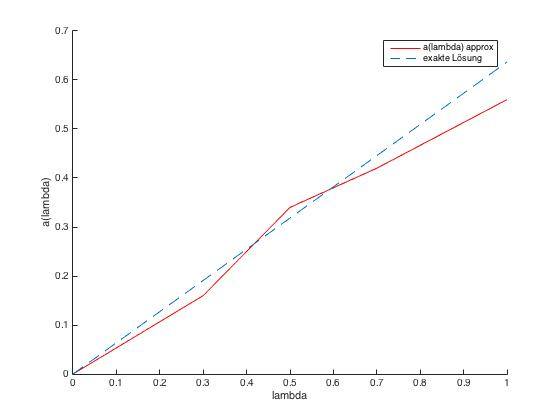
\includegraphics[width=12cm]{50.jpg}
%\caption{n=50} 
%\end{figure}

\begin{figure}[H]
\centering
%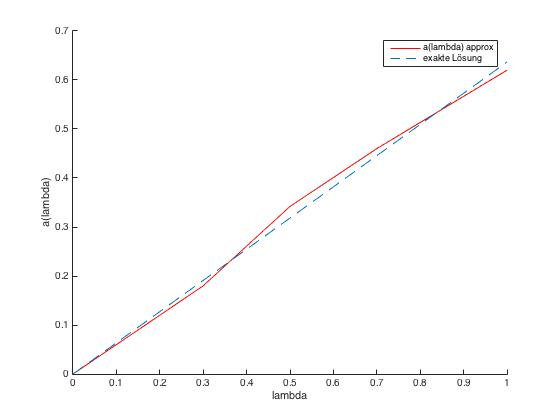
\includegraphics[width=12cm]{500.jpg}
%\caption{n=500}
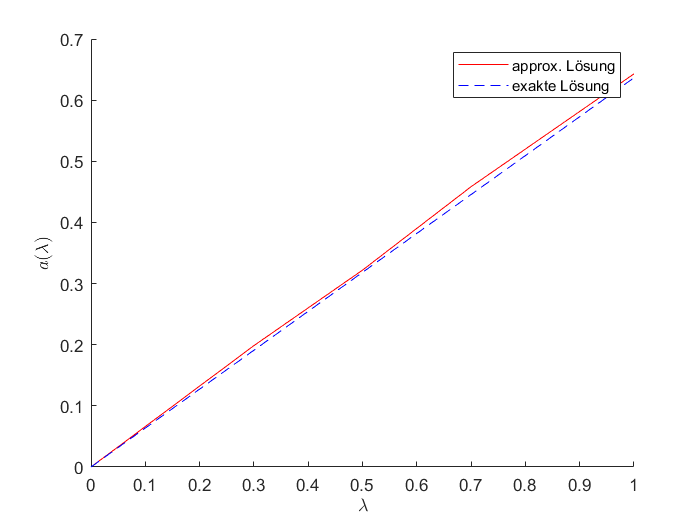
\includegraphics[width=12cm]{2000.png}
\caption{n=2000}
\end{figure}
Dies ist ein Plot mit den Ergebnissen aus obiger Tabelle und nur vier St"utzstellen.
Nun betrachten wir Plots mit einer gr"o"seren St"utzstellenanzahl. Genauer unterteilen wir das Intervall $[0,1]$ in $100$ gleichm"a"sig verteilte St"utzstellen.\\
Es ist zu erkennen, dass mit steigender Sampleanzahl das Ergenis deutlich besser wird und sich die Funktion der exakten L"osung $a(\lambda)$ ann"ahert.
\begin{figure}[H]
\centering
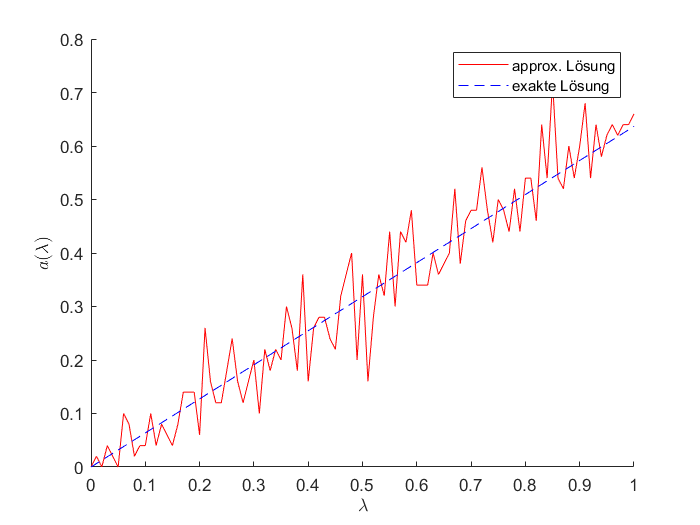
\includegraphics[width=12cm]{mc_n_50.png}
\caption{n=50}

\end{figure}
\begin{figure}[H]
\centering
%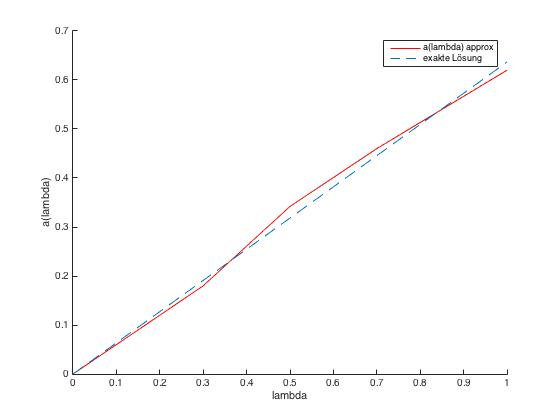
\includegraphics[width=12cm]{500.jpg}
%\caption{n=500}
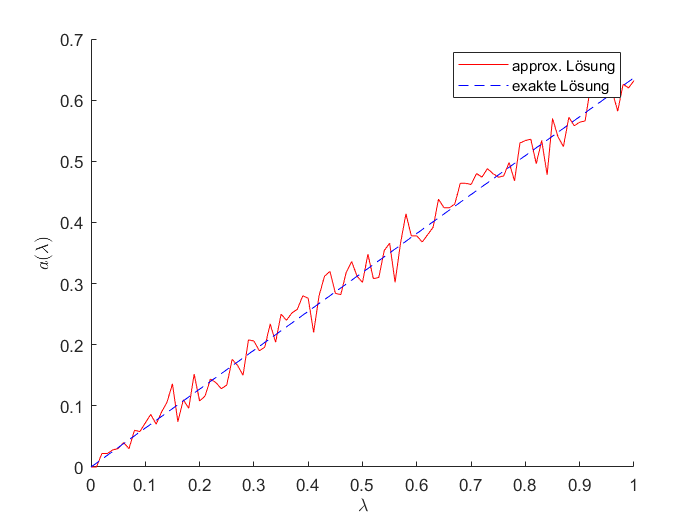
\includegraphics[width=12cm]{mc_n_500.png}
\caption{n=500}
\end{figure}

\begin{figure}[H]
\centering
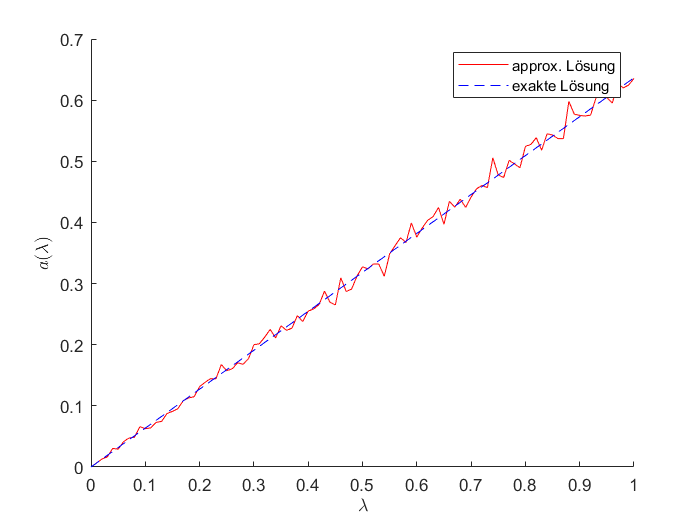
\includegraphics[width=12cm]{mc_n_2000.png}
\caption{n=2000}
\end{figure}





Mit steigender Sampleanzahl, d.h wiederholter Anzahl von Nadelw"urfen wird nat"urlich das Ergebnis besser bzw. genauer, da nach dem starken Gesetz der gro"sen Zahlen $\frac{1}{n}\sum_{i=1}^n X_i$ f"ur $n\rightarrow \infty$
fast sicher gegen $\mathbb{E}(X_1)$ konvergiert.%\vspace{1cm}

\begin{figure}[h]
\centering
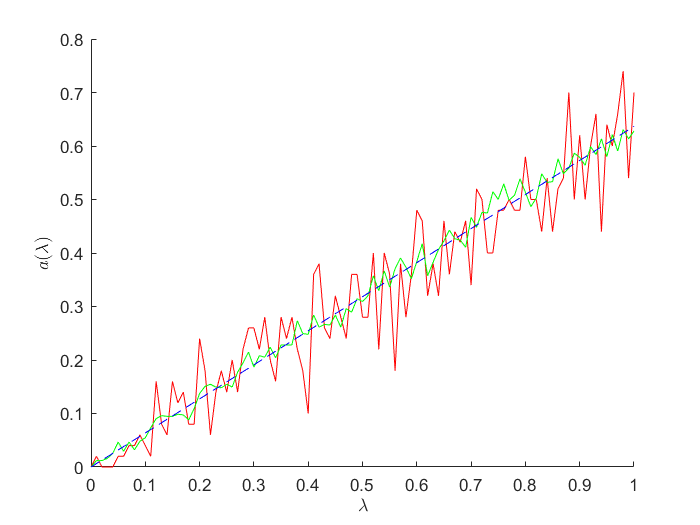
\includegraphics[width=12cm]{mc_n_50_gemittelt.png}
\caption{n=50 gemittelt}
\end{figure}

Bei obigem Plot beschreibt der gr"une Graph den Durchschnitt aus 15 Ausf"uhrungen an jeder St"utzstelle.\vspace{0.3cm}

Verwenden wir nun aber die Ergebnisse aus Proposition 3.1 Das bedeutet, wir geben uns eine Fehlerschranke $\varepsilon$ und $\theta$ vor und schauen, welches $L_\theta$ und welche Sampleanzahl uns geliefert werden. Die letzte Spalte der jeweiligen Tabellen enth"alt den tats"achlichen Fehler nach Gleichung (2).\\
Es ist in allen F"allen zu erkennen, dass der tats"achliche Fehler weit unter der vorgegebenen Schranke $\varepsilon$ liegt. Dies liegt daran, dass wir sowohl $L_\theta$ als auch $n_\theta$ aufrunden.
Weiterhin gilt nat"urlich, dass eine kleinere Fehlerschranke automatisch eine h"ohere Sampleanzahl und eine feinere Diskretisierung fordert.\\[0,2cm]
F"ur diese Tabelle gilt $\theta=0,3$.
\begin{center}
\begin{tabular}{c|c|c|c}
Fehlerschranke $\varepsilon$ & $n_\theta$ & $L_\theta$ & $\|a-\mathcal{M}_L^{\text{MC}}(n)\|_{L^2(\Omega,H)}$\\
\hline
$10^{-1}$  &  $2.81 \cdot 10^{1}$ &   $3$  &  $9.11 \cdot 10^{-3}$ \\
$10^{-2}$    & $2.63 \cdot 10^{3}$ &   $7$  &  $7.82 \cdot 10^{-5}$  \\
$10^{-3}$    & $2.62 \cdot 10^{5}$  &  $10$  &  $8.29 \cdot 10^{-7}$  \\
$10^{-4}$    &  $2.62 \cdot 10^{7}$ &   $13$  &  $9.01 \cdot 10^{-9}$ \\
$10^{-5}$ &   $2.62 \cdot 10^{9}$ &   $17$ &   $7.79 \cdot 10^{-11}$ \\
$10^{-6}$&   $2.62 \cdot 10^{11}$  &  $20$  &  $8.23 \cdot 10^{-13}$ \\ 
\hline 
 \end{tabular}
 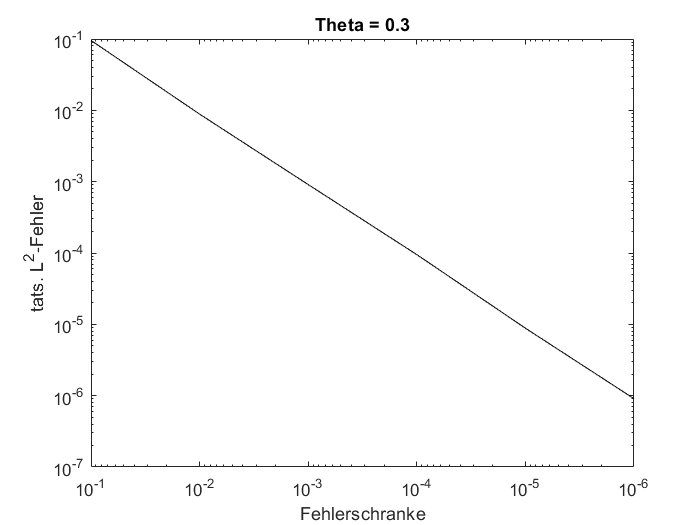
\includegraphics[width=12cm]{Plot1.png}
\end{center} 
\newpage
Hier gilt $\theta=0,5$.\\
\begin{center}
\begin{tabular}{c|c|c|c}
Fehlerschranke $\varepsilon$ & $n_\theta$ & $L_\theta$ & $\|a-\mathcal{M}_L^{\text{MC}}(n)\|_{L^2(\Omega,H)}$\\
\hline
$10^{-1}$  &  $3.93 \cdot 10^{1}$ &   $3$  &  $7.11 \cdot 10^{-3}$ \\
$10^{-2}$    & $3.7 \cdot 10^{3}$ &   $6$  &  $8.3 \cdot 10^{-5}$  \\
$10^{-3}$    & $3.67 \cdot 10^{5}$  &  $10$  &  $6.29 \cdot 10^{-7}$  \\
$10^{-4}$    &  $3.66 \cdot 10^{7}$ &   $13$  &  $7.01 \cdot 10^{-9}$ \\
$10^{-5}$ &   $3.66 \cdot 10^{9}$ &   $16$ &   $8.15 \cdot 10^{-11}$ \\
$10^{-6}$&   $3.66 \cdot 10^{11}$  &  $19$  &  $9.91 \cdot 10^{-13}$ \\ 
\hline 
 \end{tabular}\\
 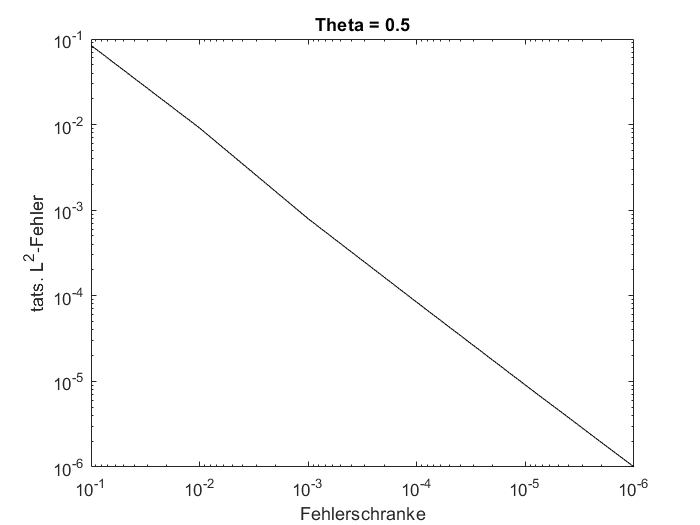
\includegraphics[width=14cm]{Plot2.png}
 \end{center}\newpage
Hier gilt $\theta=0,7$.
\begin{center}
\begin{tabular}{c|c|c|c}
Fehlerschranke $\varepsilon$ & $n_\theta$ & $L_\theta$ & $\|a-\mathcal{M}_L^{\text{MC}}(n)\|_{L^2(\Omega,H)}$\\
\hline
$10^{-1}$  &  $6.55 \cdot 10^{1}$ &   $3$  &  $5.11 \cdot 10^{-3}$ \\
$10^{-2}$    & $6.17 \cdot 10^{3}$ &   $6$  &  $6.3 \cdot 10^{-5}$  \\
$10^{-3}$    & $6.11 \cdot 10^{5}$  &  $9$  &  $8.15 \cdot 10^{-7}$  \\
$10^{-4}$    &  $6.1 \cdot 10^{7}$ &   $13$  &  $5.01 \cdot 10^{-9}$ \\
$10^{-5}$ &   $6.1 \cdot 10^{9}$ &   $16$ &   $6.15 \cdot 10^{-11}$ \\
$10^{-6}$&   $6.11 \cdot 10^{11}$  &  $19$  &  $7.91 \cdot 10^{-13}$ \\ 
\hline 
 \end{tabular}\\
 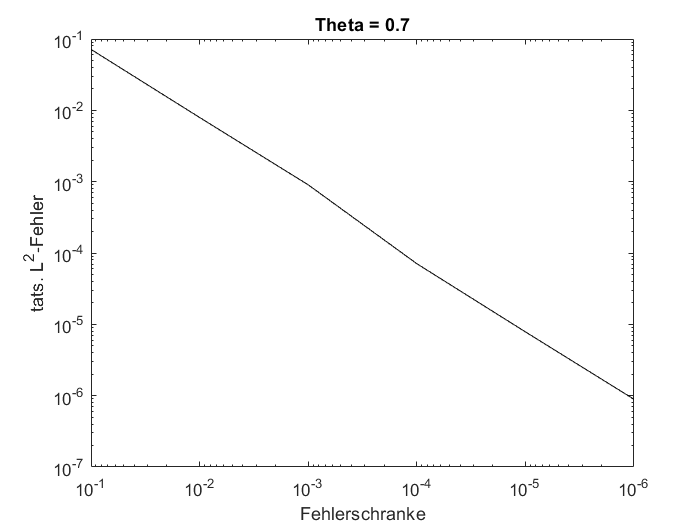
\includegraphics[width=14cm]{Plot3.png}
\end{center}

